% !TEX TS-program = pdflatex
% !TEX encoding = UTF-8 Unicode

% This is a simple template for a LaTeX document using the "article" class.
% See "book", "report", "letter" for other types of document.

\documentclass[11pt]{article} % use larger type; default would be 10pt

\usepackage[utf8]{inputenc} % set input encoding (not needed with XeLaTeX)

%%% Examples of Article customizations
% These packages are optional, depending whether you want the features they provide.
% See the LaTeX Companion or other references for full information.

%%% PAGE DIMENSIONS
%\usepackage{geometry} % to change the page dimensions
\usepackage[a4paper,left=2.5cm,right=2.5cm,bottom=2.5cm,top=2.5cm]{geometry}
\usepackage{hyperref}
% \geometry{margin=2in} % for example, change the margins to 2 inches all round
% \geometry{landscape} % set up the page for landscape
%   read geometry.pdf for detailed page layout information

\usepackage{graphicx} % support the \includegraphics command and options
\usepackage{multirow}

% \usepackage[parfill]{parskip} % Activate to begin paragraphs with an empty line rather than an indent

%%% PACKAGES
\usepackage{booktabs} % for much better looking tables
\usepackage{array} % for better arrays (eg matrices) in maths
\usepackage{paralist} % very flexible & customisable lists (eg. enumerate/itemize, etc.)
\usepackage{verbatim} % adds environment for commenting out blocks of text & for better verbatim
\usepackage{subfig} % make it possible to include more than one captioned figure/table in a single float
% These packages are all incorporated in the memoir class to one degree or another...

\usepackage{amsfonts}

%%% HEADERS & FOOTERS
\usepackage{fancyhdr} % This should be set AFTER setting up the page geometry
\pagestyle{fancy} % options: empty , plain , fancy
\renewcommand{\headrulewidth}{0pt} % customise the layout...
\lhead{}\chead{}\rhead{}
\lfoot{}\cfoot{\thepage}\rfoot{}

%%% SECTION TITLE APPEARANCE
\usepackage{sectsty}
\allsectionsfont{\sffamily\mdseries\upshape} % (See the fntguide.pdf for font help)
% (This matches ConTeXt defaults)

%%% ToC (table of contents) APPEARANCE
\usepackage[nottoc,notlof,notlot]{tocbibind} % Put the bibliography in the ToC
\usepackage[titles,subfigure]{tocloft} % Alter the style of the Table of Contents
\renewcommand{\cftsecfont}{\rmfamily\mdseries\upshape}
\renewcommand{\cftsecpagefont}{\rmfamily\mdseries\upshape} % No bold!
\usepackage{mathtools}

%%% END Article customizations

%%% The "real" document content comes below...

\title{Notes on Automatic Differentiation and \\ Differentiable Programming}
\author{Giulia Giusti}
\date{} % Activate to display a given date or no date (if empty),
        % otherwise the current date is printed 

\begin{document}
\maketitle
\tableofcontents
\newpage

\section{Automatic Differentiation in Machine Learning: a Survey}
Derivatives, mostly in the form of gradients and Hessians, are ubiquitous in machine learning. Automatic differentiation (AD) is a family of techniques similar to but more general than backpropagation for efficiently and accurately evaluating derivatives of numeric functions expressed as computer programs. Until
very recently, the fields of machine learning and AD have largely been unaware of each other and, in some cases, have independently discovered each other’s results. Despite its relevance, general-purpose AD has been missing from the machine learning toolbox, a situation slowly changing with its ongoing adoption under the names \emph{dynamic computational graphs} and \emph{differentiable programming}.

\subsection{Introduction}
Methods for the computation of derivatives in computer programs can be classified into four categories:
\begin{center}
\begin{tabular}{|c|l|l|} 
\hline
 Method & Pros & Cons\\
\hline
 Manual Differentiation & & -Time consuming \\ 
 & & -Error prone\\ \hline
 Numerical Differentiation& Easier to implement & -Highly inaccurate due to round-off\\
 & than the manual  & and truncation errors\\
 & method & -Scales poorly for gradients\\ 
 & & ($\Rightarrow$ inappropriate for machine learning) \\ \hline
 Symbolic Differentiation & Addresses the weaknesses & Often results in complex and cryptic  \\ 
 & of both the manual & expressions plagued with the problem \\ 
 & and  numerical methods & of \emph{expression swell}\\ \hline
\end{tabular}
\end{center}
\vspace{5mm}
\noindent Furthermore, manual and symbolic methods require models to be defined as closed-form expressions, ruling out or severely limiting algorithmic control flow and expressivity.
\newline 

The last and most powerful method is represented by \emph{Automatic Differentiation (AD)} which performs a non-standard interpretation of a given computer program by replacing the domain of the variables to incorporate derivative values and redefining the semantics of the operators to propagate derivatives per the chain rule of differential calculus. We would like to stress that AD as a technical term refers to a specific family of techniques that compute derivatives through accumulation of values during code execution to generate numerical derivative evaluations rather than derivative expressions. This allows accurate evaluation of derivatives at machine precision with only a small constant factor of overhead and ideal asymptotic efficiency.

In contrast with the effort involved in arranging code as closed-form expressions under the syntactic and semantic constraints of symbolic differentiation, AD can be applied to regular code with minimal change, allowing branching, loops, and recursion. 
\newline 

In machine learning, a specialized counterpart of AD known as the backpropagation algorithm has been the mainstay for training neural networks, with a colorful history of having been reinvented at various times by independent researchers. In simplest terms, backpropagation models learning as gradient descent in neural network weight space, looking for the minima of an objective function. The required gradient is obtained by the backward propagation of the sensitivity of the objective value at the output, utilizing the chain rule to compute partial derivatives of the objective with respect to each weight. The resulting algorithm is essentially equivalent to transforming the network evaluation function composed with the objective function under reverse mode AD, which, as we shall see, actually generalizes the backpropagation idea.

\subsection{What AD Is Not}
Without proper introduction, one might assume that AD is either a type of numerical or symbolic differentiation. Confusion can arise because AD does in fact provide numerical values of derivatives (as opposed to derivative expressions) and it does so by using symbolic rules of differentiation (but keeping track of derivative values as opposed to the resulting expressions), giving it a two-sided nature that is partly symbolic and partly numerical.

\subsubsection{AD Is Not Numerical Differentiation}
Numerical differentiation is the finite difference approximation of derivatives using values of the original function evaluated at some sample points. In its simplest form, it is based on the limit definition of a derivative. For example, for a multivariate function $f:\mathbb{R}^n\rightarrow \mathbb{R}$ one can approximate the gradient $\nabla f = (\frac{\partial f}{\partial x_1},...,\frac{\partial f}{\partial x_n})$ using
$$ \frac{\partial f (x)}{\partial x_i} \approx \frac{f(x+he_i)-f(x)}{h} $$
where $e_i$ is the i-th unit vector (it is used to modify only the i-th direction of the point x) and $h>0$ is a small step size.

Let's summarize the pros and cons of numerical differentiation with the following table:

\begin{center}
\begin{tabular}{ |l|l| } 
\hline
 Pros & Cons\\
\hline
Simple to implement & -O(n) evaluations of $f$ for a gradient in $n$ dimensions \\ 
 & -Careful selection of the step size $h$ \\ \hline
\end{tabular}
\end{center}
Numerical approximations of derivatives are inherently ill-conditioned and unstable  because using the limit definition of the derivative for finite difference approximation then one commits both cardinal sins of numerical analysis: “thou shalt not add small numbers to big numbers”, and “thou shalt not subtract numbers which are approximately equal”. This is due to the introduction of truncation and round-off errors inflicted by the limited precision of computations and the chosen value of the step size $h$. Truncation error tends to zero as $h \rightarrow 0$. However, as $h$ is decreased, round-off error increases and becomes dominant.

\paragraph{Numerical Differentiation and ML} The major obstacle to applying numerical differentiation to machine learning is the complexity O(n), because $n$ can be as large as millions or billions in state-of-the-art deep learning models. In contrast, approximation errors would be tolerated in a deep learning setting thanks to the well-documented error resiliency of neural network architectures.

\subsubsection{AD Is Not Symbolic Differentiation}
Symbolic differentiation is the automatic manipulation of expressions for obtaining derivative expressions, it is carried out by applying transformations representing rules of differentiations such as
$$ \frac{d}{dx}(f(x)+g(x)) \rightarrow \frac{d}{dx} f(x) + \frac{d}{dx} g(x) $$
$$ \frac{d}{dx}(f(x)\cdot g(x))\rightarrow \bigg( \frac{d}{dx} f(x) \bigg) g(x) + f(x) \bigg( \frac{d}{dx} g(x) \bigg) $$
\noindent When formulae are represented as data structures, symbolically differentiating an expression tree is a perfectly mechanistic process. 

Let's summarize the pros and cons of numerical differentiation with the following table:

\begin{center}
\begin{tabular}{ |l|l| } 
\hline
 Pros & Cons\\
\hline
In optimization, symbolic derivatives can & No efficient runtime calculation of derivative  \\
give valuable insight into the structure of & values because symbolic expression can get \\ 
the problem domain and produce analytical & exponentially larger than the expression   \\
 solution of extrema that can eliminate the & whose derivative they represent.\\ 
need for derivative calculation altogether.  & \\ \hline
\end{tabular}
\end{center}

\paragraph{Automatic differentiation Solution} Automatic differentiation tries to solve the efficiency problem of Symbolic Differentiation. When we are concerned with the accurate numerical evaluation of derivatives and not so much with their actual symbolic form, it is in principle possible to significantly simplify computations by storing only the values of intermediate sub-expressions in memory. Moreover, for futher efficiency, we can interleave as much as possible the differentiation and simplification steps. This interleaving idea forms the basis of AD and provides an account of its simplest form: \textit{apply symbolic differentiation at the elementary operation level and keep intermediate numerical results, in lockstep with the evolution of the main function.}

\subsection{AD and Its Main Modes}
AD can be thought as performing a non-standard interpretation of a computer program where this interpretation involves augmenting the standard computation with the calculation of various derivatives. All numerical computations are ultimately compositions of a finite set of elementary operations for which derivatives are known and combining the derivatives of the constituent operations through the chain rule gives the derivative of the overall composition.

Given a function $f: \mathbb{R}^n \rightarrow \mathbb{R}^m$, an \emph{evolution trace} is constructed using intermediate variables $v_i$ such that
\begin{itemize}
	\item variables $v_{i-n}=x_i$, $i=1,...,n$ are the input variables,
	\item variables $v_{i} \mbox{ } i$, $i=1,...,l$ are the working (intermediate) variables, and
	\item variables $y_{m-i}=v_{l-i}$, $i=m-1,...,0$ are the output variables.
\end{itemize}

\paragraph{Example} Let us consider the function $f(x_1,x_2)= ln(x_1)+ x_1 \cdot x_2 -sin(x_2)$. The computational graph of this function is the following

\begin{figure}[h!]
	\centering
	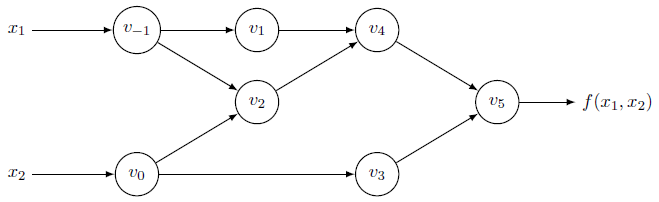
\includegraphics[scale=0.9]{img/compGraph}
	\caption{Computational graph of the function $f(x_1,x_2)= ln(x_1)+ x_1 \cdot x_2 -sin(x_2)$}
	\label{compGraph}
\end{figure}
\noindent This graph is useful for visualizing dependency relationships between intermediate variables. We will see in the next sections the evolution traces for forward mode and reverse mode related to this example.

\vspace*{4mm}
An important point to note here is that AD can differentiate not only closed-form expressions in the classical sense, but also algorithm making use of control flow such as branching, loops, recursion, and procedure calls, giving it an important advantage over symbolic differentiation which severely limits such expressivity. This is thanks to the fact that any numeric code will eventually result in a numeric evaluation trace with particular values of the input, intermediate, and output values, which are the only things one needs to know for computing derivatives using chain rule composition, regardless of the specific control flow path that was taken during execution.

\subsubsection{Forward Mode}
AD in forward accumulation mode is the conceptually most simple type.

\paragraph{Example}
Let us consider the evalutation trace of the function $f(x_1,x_2)= ln(x_1)+ x_1 \cdot x_2 -sin(x_2)$ give on the left-hand side in Figure~\ref{evalTrace} and in graph form in Figure~\ref{compGraph}. In order to compute the derivative of $f$ with respect to $x_1$, we start by associating with each intermediate variable $v_i$ a derivative $\dot{v_i}=\frac{\partial v_i}{\partial x_1}$. Then applying the chain rule to each elementary operation in the forward primal trace, we generate the corrisponding tangent derivative trace, given on the right-hand side in Figure~\ref{evalTrace}. Evaluating the primals $v_i$ in lockstep with their corrisponding tangent $\dot{v_i}$ gives us the required derivative in the final variable $\dot{v_5}=\frac{\partial y}{\partial x_1}$.

\begin{figure}[h!]
	\centering 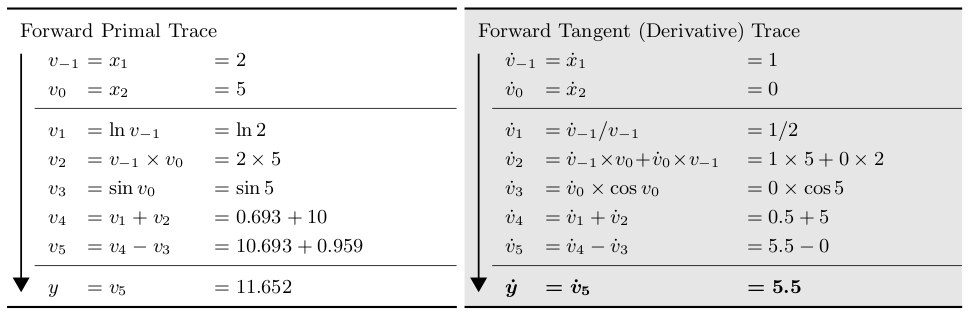
\includegraphics[scale=0.47]{img/evalTrace}
	\caption{Forward mode AD example, with $y=f(x_1,x_2)= ln(x_1)+ x_1 \cdot x_2 -sin(x_2)$ evaluated at $(x_1, x_2)=(2,5)$ and setting $\dot{x_1}=1$ to compute $\frac{\partial y}{\partial x_1}$.}
	\label{evalTrace}
\end{figure}

\subsubsection{Reverse Mode}
AD in the reverse accumulation mode corresponds to a generalized backpropagation algorithm, in that it propagates derivatives backward from a given output. This is done by complementing each intermediate variable $v_i$ with an adjoint $\overline{v}_i=\frac{\partial y_j}{\partial v_i}$ which represents the sensitivity of a considered output $y_j$ with respect to changes in $v_i$. In the case of backpropagation, $y$ would be a scalar corresponding to the error $E$.

In reverse mode AD, derivatives are computed in the second phase of a two-phase process. In the first phase, the original function code is run forward, populating intermediate variables $v_i$ and recording the dependencies in the computational graph through a book-keeping procedure. In the second phase, derivatives are calculated by propagating adjoints
$\overline{v}_i$ in reverse, from the outputs to the inputs.

\paragraph{Backpropagation Algorithm}
After performing the forward pass through the network, we need to calculate the loss function which is used to calculate the distance between the predicted value and the actual value. Backpropagation aims to minimize the cost function by adjusting network’s weights and biases. The level of adjustment is determined by the gradients of the loss function with respect to those parameters. Compute those gradients happens using a technique called \emph{chain rule}.

\paragraph{Example}
Returning to the example $y=f(x_1,x_2)= ln(x_1)+ x_1 \cdot x_2 -sin(x_2)$, in Figure~\ref{revMode}  we see the adjoint statements on the right-hand side, corresponding to each original elementary operation on the left-hand side.

\begin{figure}[h!]
	\centering 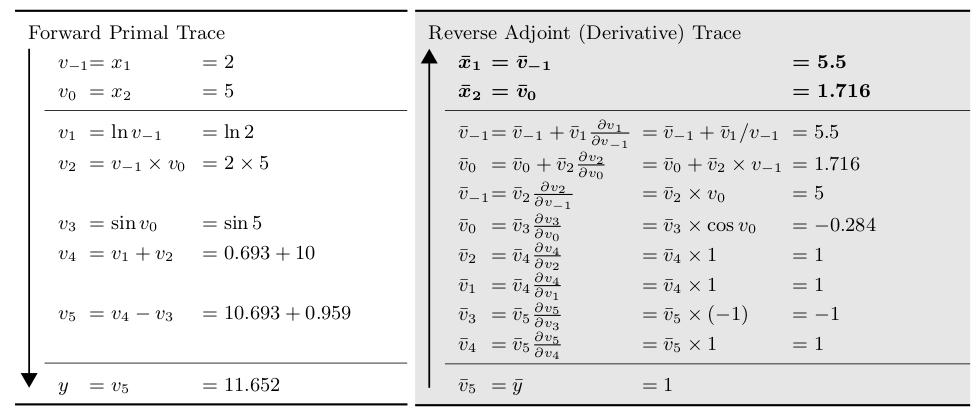
\includegraphics[scale=0.47]{img/revMode}
	\caption{Reverse mode AD example with $y=f(x_1,x_2)= ln(x_1)+ x_1 \cdot x_2 -sin(x_2)$ evaluated at $(x_1,x_2)=(2,5)$. After the forward evaluation of the primals on the left, the adjoint operations on the right are evaluated in reverse. Note that both $\overline{x}_1=\frac{\partial y}{\partial x_1}$ and $\overline{x}_2=\frac{\partial y}{\partial x_2}$ are computed in the same reverse pass, starting from the adjoint  $\overline{v}_5=\overline{y}=\frac{\partial y}{\partial y}=1$.}
	\label{revMode}
\end{figure}

In simple terms, we are interested in computing the contribution $\overline{v}_i=\frac{\partial y_j}{\partial v_i}$ of the change in each variable $v_i$ to the change in the output $y$. Taking the variable $v_0$ as an example, we see in Figure~\ref{compGraph} that the only way it can affect $y$ is through affecting $v_2$ and $v_3$ , so its contribution to the change in $y$ is given by
$$ 
	\frac{\partial y}{\partial v_0} = \frac{\partial y}{\partial v_2} \frac{\partial v_2}{\partial v_0} +\frac{\partial y}{\partial v_3} \frac{\partial 		v_3}{\partial v_0}
$$
\noindent where $\overline{v}_2=\frac{\partial y}{\partial v_2}$ and  $\overline{v}_3=\frac{\partial y}{\partial v_3}$. In Figure~\ref{revMode} , this contribution is computed in two incremental steps
$$
	\overline{v}_0=\overline{v}_3 \frac{\partial v_3}{\partial v_0} \quad \quad\quad\quad\quad \overline{v}_0= \overline{v}_0 + \overline{v}_2 \frac{\partial 		v_2}{\partial v_0}
$$
lined up with the lines in the forward trace from which these expressions originate.

After the forward pass on the left-hand side, we run the reverse pass of the adjoints on the right-hand side, starting with $\overline{v}_5=\overline{y}=\frac{\partial y}{\partial y}=1$. In the end we get the derivatives $\overline{x}_1=\frac{\partial y}{\partial x_1}$ and $\overline{x}_2=\frac{\partial y}{\partial x_2}$ in just one reverse pass.

\paragraph{Forward Mode Advantage}
An important advantage of the reverse mode is that it is significantly less costly to evaluate (in terms of operation count) than the forward mode for functions with a large number of inputs. In the extreme case of $f: \mathbb{R}^n \rightarrow \mathbb{R}$, only one application of the reverse mode is sufficient to compute the full gradient $\nabla f = \bigg( \frac{\partial y}{\partial x_1},..., \frac{\partial y}{\partial x_n}\bigg)$, compered with the $n$ passes of the forward mode needed for populating the same. Because machine learning
practice principally involves the gradient of a scalar-valued objective with respect to a large number of parameters, this establishes the reverse mode, as opposed to the forward mode, as the mainstay technique in the form of the backpropagation algorithm.

\subsection{AD and Machine Learning}
Areas where AD has seen use include optimization, neural networks, computer vision, natural language processing, and probabilistic inference.

\subsubsection{Gradient-Based Optimization}
Gradient-based optimization is one of the pillars of machine learning. Given an objective function $f: \mathbb{R}^n \rightarrow \mathbb{R}$, classical gradient descent has the goal of finding (local) minima $\mathbf{w}^* = argmin_{\mathbf{w}} f(\mathbf{w})$ via updates of the form $\Delta  \mathbf{w} = -\eta \nabla f$ where $\eta >0$ is a step size (known as \emph{learning rate}). Gradient-based methods make use of the fact that $f$ decreases steepest if one goes in the direction of the negative gradient. The convergence rate of gradient-based methods is usually improved by adaptive step-size techniques that adjust the step size $\eta$ on every iteration. As we have seen, for large $n$, reverse mode AD provides a highly efficient method for computing gradients.

\subsubsection{Neural Networks, Deep Learning, Differentiable Programming}
Training of a neural network is an optimization problem with respect to its set of weights, which can in principle be addressed by using any method ranging from evolutionary algorithms to gradient-based methods  or the mainstay stochastic gradient descent and its many variants.

As we have seen, the backpropagation algorithm is only a special case of AD: \textit{by applying reverse mode AD to an objective function evaluating a network’s error as a function of its weights, we can readily compute the partial derivatives needed for performing weight updates}.

In mainstream frameworks including Theano, TensorFlow, Caffe, and CNTK the user first constructs a model as a computational graph using a domain-specific mini language, which then gets interpreted by the framework during execution. This approach has the advantage of enabling optimizations of the computational graph structure, but the disadvantages of having limited and unintuitive control flow and being difficult to debug. In contrast, the lineage of recent frameworks led by autograd, Chainer, and PyTorch provide truly general-purpose reverse mode AD,
where the user directly uses the host programming language to define the model as a regular program of the forward computation. This eliminates the need for an interpreter, allows arbitrary control flow statements, and makes debugging simple and intuitive.

Simultaneously with the ongoing adoption of general-purpose AD in machine learning, we are witnessing a modeling-centric terminology emerge within the deep learning community. The terms \emph{define-and-run} and \emph{static computational graph} refer to Theano-like systems where a model is constructed, before execution, as a computational graph structure, which later gets executed with different inputs while remaining fixed. In contrast, the terms \emph{define-by-run} and \emph{dynamic computational graph} refer to the general-purpose AD capability available in newer PyTorch-like systems where a model is a regular program in the host programming language, whose execution dynamically constructs a computational graph on-the-fly that can freely change in each iteration.

\emph{Differentiable Programming} is another emerging term referring to the realization that deep learning practice essentially amounts to writing program templates of potential solutions to a problem, which are constructed as differentiable directed graphs assembled from functional blocks whose parameters are learned from examples using gradient-based optimization. Expressed in this paradigm, neural networks are just a class of parameterized
differentiable programs composed of building blocks such as feed-forward, convolutional, and recurrent elements.

























\newpage

\section{Backpropagation in the Simply Typed Lambda-Calculus with Linear Negation}
Backpropagation is a classic automatic differentiation algorithm computing the gradient of functions specified by a certain class of simple, first-order programs, called \emph{computational graphs}. 
Recent years have witnessed the quick growth of a research field called \emph{differentiable programming}, the aim of which is to express computational graphs more synthetically and modularly by resorting to actual programming languages endowed with control flow operators and higher-order combinators, such as map and fold. In this paper, we extend the backpropagation algorithm to a paradigmatic example of such a programming language: we define a compositional program transformation from the simply-typed lambda-calculus to itself augmented with a notion of linear negation, and prove that this computes the gradient of the source program with the same efficiency as first-order backpropagation.

\subsection{Introduction}
In the past decade there has been a surge of interest in so-called deep learning, a class of machine learning methods based on multi-layer neural networks. The term “deep” has no formal meaning, it is essentially a synonym of “multi-layer”, which refers to the fact that the networks have, together with their input and output layers, at least one internal (or “hidden”) layer of artificial neurons. Technically, the neurons are just functions $\mathbb{R}^n \rightarrow \mathbb{R}$ of the form $(x_1,..., x_m) \rightarrow \sigma(\sum^{m}_{i=1} w_i \cdot x_i)$, where $\sigma: \mathbb{R}\rightarrow\mathbb{R}$ is some \emph{activation function} and $w_1,..., w_m \in \mathbb{R}$ are the \emph{weights} of the neuron.

Feed-forward, multi-layer neural networks are known to be universal approximators: any continuous function $f: K \rightarrow \mathbb{R}$ with $K \subset \mathbb{R}^k$ compact may be approximated to an arbitrary degree of precision by a feed-forward neural network with one hidden layer, as long as the weights are set properly. This leads us to the following two questions related to each other:
\begin{enumerate}
	\item How to efficiently train a neural network? i.e., how to find the right weights as quickly as possible?
	\item How to select and, if necessary, modify or design network architectures adapted to a given task?
	Since the quality of an architecture is also judged in terms of training efficiency, this problem is actually interlaced
	with the previous one.
\end{enumerate}

\subsubsection{How to efficiently train a neural network?} The first question is generally answered in terms of the gradient descent algorithm (or some variant thereof). 

\paragraph{Gradient Descent Algorithm} The Gradient Descent Algorithm finds local minima of a function $G : \mathbb{R}^n \rightarrow \mathbb{R}$ using its gradient $\nabla G$. The algorithm starts by choosing a point $\mathbf{w}_0 \in \mathbb{R}^n$. Under certain assumptions, if $\nabla G(\mathbf{w}_0)$ is close to zero then $\mathbf{w}_0$ is within a sufficiently small neighborhood of a local minimum. Otherwise, we know that $G$ decreases most sharply in the opposite direction of $\nabla G(\mathbf{w}_0)$, and so the algorithm sets $\mathbf{w}_1 := \mathbf{w}_0 - \rho \nabla G(\mathbf{w}_0)$ for a suitable step rate $\rho >0$, and repeats the procedure from $\mathbf{w}_1$ .

\paragraph{AD and efficient training of neural networks} So, regardless of the architecture, efficiently training a neural network involves efficiently computing gradients. The interest of gradient descent, however, goes well beyond deep learning, into fields such as physical modeling and engineering design optimization, each with numerous applications. It is thus no wonder that a whole research fie
known as automatic differentiation (AD for short), developed around the computation of gradients. In AD, the setting of neural networks is generalized to computational graphs, which are arbitrarily complex compositions of nodes computing basic functions and in which the output of a node may be shared as the input of an unbounded number of nodes.

The key idea of AD is to compute the gradient of a computational graph by accumulating in a suitable way the
partial derivatives of the basic functions composing the graph. This rests on the mathematical principle known as
\emph{chain rule}, giving the derivative of a composition $f \circ g$ from the derivatives of its components $f$ and $g$. Formally, the chain rule states that

$$\forall r \in \mathbb{R} \quad \quad (g \circ f)' (r) = g'(f(r)) \cdot f'(r)$$

There are two main “modes” of applying this rule in AD, either forward, propagating derivatives from inputs to outputs, or backwards, propagating derivatives from outputs to inputs. If $G$ is a computational graph with $n$ inputs and $m$ outputs invoking $|G|$ operations, forward mode computes the Jacobian of $G$ in $O(n |G|)$ operations, while reverse mode requires $O(m |G|)$ operations. In deep learning, as the number of layers increases, $n$ becomes astronomical (millions, or even billions) while $m = 1$, hence the reverse mode is the method of choice and specializes in what is called the backpropagation algorithm. Today, AD techniques are routinely used in the industry through deep learning frameworks such as TensorFlow and PyTorch.


\subsubsection{How to select and modify or design network architectures adapted to a given task?}
The interest of the programming languages (PL) community in AD stems from the second deep learning question mentioned above, namely the design and manipulation of (complex) neural network architectures. As it turns out, these are being expressed more and more commonly in terms of actual programs. Although these programs always reduce, in the end, to computational graphs, these latter are inherently static and therefore inadequate to properly describe something which is in reality, a dynamically-genereted neural network.

In PL-theoretic terms, this amounts to fixing a reduction strategy, which cannot always be optimal in terms of efficiency. There is also a question of modularity: if gradients may only be computed by running programs, then we are implicitly rejecting the possibility of computing gradients modularly, because a minor change in the code might result in having to recompute everything from scratch, which is clearly unsatisfactory.

\subsubsection{Goal}
Define a compositional program trasformation $\stackrel{\leftarrow}{D}$ extending the backpropagation algorithm from computational graph to general simply typed $\lambda$-terms. Our framework is purely logical and therefor offer the possibility of importing tool from semantics, type systems and rewriting theory.

\subsection{A Crash Course in Automatic Differentiation}

\subsubsection{What is Automatic Differentiation?}
Automatic differentiation (or AD) is the science of efficientlly computing the derivative of (a restricted class of) programs. Such programs may be represented as directed acyclic hypergraphs, called \emph{computational graphs}, whose nodes are variables of type $\mathbb{R}$ and whose hyperedges are labelled by functions drawn from some finite set of interest with the restriction that hyperedges have exactly one targetnode and that each node is the target of at most one hyperedge. The basic idea is that nodes that are not target of any hyperedge represent input variables, nodes which are not source of any hyperedge represent outputs, and a hyperedge $x_1, \dots, x_k \xrightarrow{f} y$ represents an assignment $y:= f(x_1,\dots, x_k)$. So that a computational graph with $n$ inputs and $m$ outputs represents a function of type $\mathbb{R}^n\rightarrow \mathbb{R}^m$. 

In terms of programming languages, we may define computational graphs as generated by
$$ F, G ::= x \mbox{ }|\mbox{ }  f(x_1,...,x_k) \mbox{ }|\mbox{ }  \mathtt{let} \mbox{ } x = G \mbox{ } \mathtt{in} \mbox{ }F \mbox{ }|\mbox{ }  (F,G) $$

where $x$ range over ground variables and $f$ over a set of real function symbols. The $\mathtt{let}$ binders are necessary to represents \emph{sharing}. The set of real function symbols consists of one nullary symbol for every real number plus finitely many non-nullary symbols for actual functions, we may write $f(G_1,\dots.G_n)$ as a syntactic sugar for $\mathtt{let} \mbox{ } x_1 = G_1 \mbox{ } \mathtt{in} \mbox{ } \dots \mbox{ } \mathtt{let} \mbox{ } x_n = G_n \mbox{ } \mathtt{in}  \mbox{ } f(x_1,...,x_n)$. 

\paragraph{Example} For example, the computational graph that represents the function $(x_1, x_2) \mapsto sin((x_1-x_2)^2)$ and its corresponding term are described in Figure~\ref{compGraph2}.

\begin{figure}[h!]
	\centering
	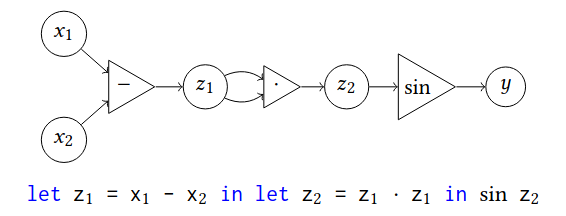
\includegraphics[scale=0.5]{img/compGraph2}
	\caption{Computational graph of the function $f(x_1,x_2)=sin((x_1-x_2)^2)$ and its corresponding term. Nodes are drawn as circles, 			hyperedges as triangles.}
	\label{compGraph2}
\end{figure}

\subsubsection{Forward Mode AD}

\subsubsection{Symbolic AD}

\subsubsection{Reverse Mode AD or Backpropagation}

\subsubsection{Symbolic Backpropagation and the Compositionality Issue}

\end{document}
